\documentclass[10pt,border=5pt]{standalone}
\usepackage[T1]{fontenc}
\usepackage{lmodern,amsmath,amssymb,mathrsfs,tikz}
\usetikzlibrary{arrows.meta,positioning,calc}
\definecolor{ink}{HTML}{192536}
\definecolor{blue}{HTML}{2E70AE}
\definecolor{gold}{HTML}{A66A15}
\definecolor{green}{HTML}{28764D}
\definecolor{red}{HTML}{B43D3D}
\newcommand{\C}{\mathbb C}
\newcommand{\R}{\mathcal R}
\newcommand{\Lr}{\mathcal L_{\mathrm{res}}}
\newcommand{\Prs}{\mathcal P_{\mathrm{res}}}
\newcommand{\Tr}{T_{\mathrm{resp}}}
\newcommand{\rr}{\rho_{\mathrm{res}}}
\tikzset{every node/.style={font=\small,text=ink,align=center},
 box/.style={draw=blue,fill=blue!4,rounded corners=3pt,line width=.7pt,inner sep=7pt},
 goldbox/.style={box,draw=gold,fill=gold!5},
 greenbox/.style={box,draw=green,fill=green!5},
 redbox/.style={box,draw=red,fill=red!4},
 edge/.style={-{Stealth[length=4pt]},draw=ink,line width=.7pt},
 heading/.style={font=\small\bfseries},
 note/.style={font=\small,text=ink!85}}

\begin{document}
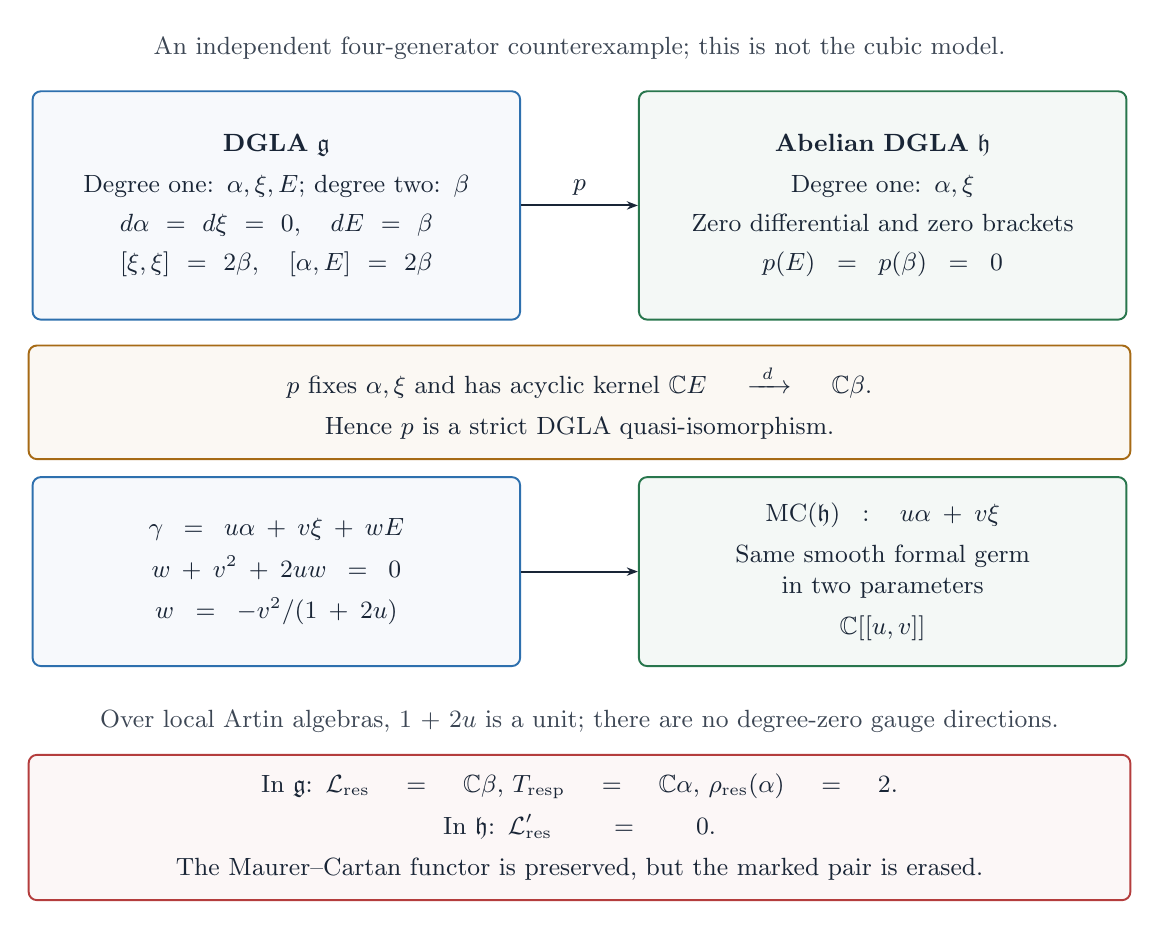
\begin{tikzpicture}
\node[note,text width=13.5cm] at (0,1)
 {An independent four-generator counterexample; this is not the cubic model.};
\node[box,text width=5.7cm,minimum height=29mm] (g) at (-3.85,-1)
 {\textbf{DGLA $\mathfrak g$}\\[4pt]
 Degree one: $\alpha,\xi,E$; degree two: $\beta$\\[3pt]
 $d\alpha=d\xi=0,\quad dE=\beta$\\[3pt]
 $[\xi,\xi]=2\beta,\quad[\alpha,E]=2\beta$};
\node[greenbox,text width=5.7cm,minimum height=29mm] (h) at (3.85,-1)
 {\textbf{Abelian DGLA $\mathfrak h$}\\[4pt]
 Degree one: $\alpha,\xi$\\[3pt]
 Zero differential and zero brackets\\[3pt]
 $p(E)=p(\beta)=0$};
\draw[edge] (g)--node[above]{$p$}(h);
\node[goldbox,text width=13.5cm] (kernel) at (0,-3.5)
 {$p$ fixes $\alpha,\xi$ and has acyclic kernel
 $\C E\xrightarrow{\ d\ }\C\beta$.\\[4pt]
 Hence $p$ is a strict DGLA quasi-isomorphism.};
\node[box,text width=5.7cm,minimum height=24mm] (mcg) at (-3.85,-5.65)
 {$\gamma=u\alpha+v\xi+wE$\\[4pt]
 $w+v^2+2uw=0$\\[4pt]
 $w=-v^2/(1+2u)$};
\node[greenbox,text width=5.7cm,minimum height=24mm] (mch) at (3.85,-5.65)
 {$\operatorname{MC}(\mathfrak h):\ u\alpha+v\xi$\\[4pt]
 Same smooth formal germ\\in two parameters\\[4pt]
 $\C[[u,v]]$};
\draw[edge] (mcg)--(mch);
\node[note,text width=13.5cm] at (0,-7.55)
 {Over local Artin algebras, $1+2u$ is a unit; there are no degree-zero gauge directions.};
\node[redbox,text width=13.5cm] at (0,-8.9)
 {In $\mathfrak g$: $\Lr=\C\beta$, $\Tr=\C\alpha$, $\rr(\alpha)=2$.\\[4pt]
 In $\mathfrak h$: $\mathcal L'_{\mathrm{res}}=0$.\\[4pt]
 The Maurer--Cartan functor is preserved, but the marked pair is erased.};
\end{tikzpicture}
\end{document}
